\documentclass[12pt, a4paper]{article}
\usepackage[italian]{babel}
\usepackage[utf8]{inputenc}
\usepackage[T1]{fontenc}

% MATEMATICA
\usepackage{amsmath}
\usepackage{amsfonts}
\usepackage{amssymb}
\usepackage{amsthm}
\usepackage{mathtools}
\usepackage{esint}
\usepackage{amsmath}
\usepackage{cancel}

% IMMAGINI E GRAFICA
\usepackage{graphicx}
\usepackage{float}
\usepackage{subcaption}
\usepackage{tikz}

% LAYOUT E FORMATTAZIONE
\usepackage{geometry}
\usepackage{fancyhdr}
\usepackage{enumitem}
\usepackage{parskip}
\usepackage{titlesec}

% TABELLE
\usepackage{array}
\usepackage{booktabs}
\usepackage{tabularx}

% CODICE (se servisse)
\usepackage{listings}
\usepackage{xcolor}

% DEFINIZIONI
\usepackage{enumitem}
\setlist[description]{
    style=nextline,
    font=\normalfont\bfseries,
    leftmargin=2cm,
    itemsep=0.5ex
}

% HYPERREF (sempre per ultimo)
\usepackage[hidelinks]{hyperref}
\usepackage{fancyhdr}
\pagestyle{fancy}
\fancyhf{}
\renewcommand{\headrulewidth}{0pt}

% Romani per le pagine prima del contenuto
\pagenumbering{Roman}


\begin{document}
% Frontespizio
\title{Elettrotecnica}
\author{Luca Pes}
\date{I Semestre, III Anno}
\maketitle

% Pagina vuota
\newpage

% Sommario con numerazione romana
\tableofcontents
\thispagestyle{fancy}

\section{Carica}
\subsection{Carica Elettrica}
    Per le cariche elettriche sono presenti due modelli matematici per descrivere la loro distribuzione dello spazio:
    \begin{itemize}
        \item Cariche puntiformi: modello discreto
        \item Distribuzione di carica: modello continuo
    \end{itemize}

    È importante definire una variabile fisica chiamata carica contenuta: è la carica contenuta in un volume v ($q^c[t,v]$ con $q^c$ funzione del volume v e si esprime in Coulomb).\\
    $q^c$ è una variabile globale, cioè dipende dalla scelta di un elemento geometrico v che descrive il volume.\\
    Si può quindi definire la densità volumica di carica $\rho_c$. Per definire questo elemento si ipotizza che la \textbf{carica si distribuisca uniformemente in v}. \\
    \begin{center}
        $\rho_c(t,p) := \frac{q^c[t,v]}{v}, \rho \in v [\frac{C}{m^3} ]$\\
    \end{center}
    Come è logico pensare, la carica solitamente \textbf{NON} si distribuisce uniformemente.

    \subsubsection{Principio di uniformità}
        INSERIRE GRAFICO\\
        Se si considera un intervallo infinitesimo in un intorno del punto P, anche la variazione della funzione in quell'intorno sarà infinitesima. Per grandezze infinitesime, quindi, si può assumere che le grandezze siano uniformi e costanti.

        Applicando il \textbf{principio di uniformità} alla determinazione di $\rho_c$ ne caso generale:
        \begin{enumerate}
            \item prendiamo un punto $P \in v$
            \item prendiamo un \textbf{cubo centrato in P}
            \item $\lim_{v' \to 0} \rightarrow 0$
            \item nel $v'$ la carica si distribuisce uniformemente
            \item applichiamo la definizione di $\rho_c$ nel caso di distribuzione uniforme a $v'$\\
            \begin{equation}
                \rho_c[t,P] := \lim_{v' \to 0} \frac{q^c[t,v']}{v'} = \frac{dq(t,p)}{dv}
            \end{equation}
            \item effettuare la stessa procedura per qualsiasi punto dentro v
        \end{enumerate}

Si ottiene così un \textbf{campo scalare} $\rho_c(t,\mathbf{P})$: per ogni punto $\mathbf{P} \in V$, $\rho_c$ restituisce uno scalare (densità volumetrica). All'interno di un volume:
\[
q^c[t,\tau] = \int_\tau \rho_c(t,\mathbf{P}) \, dv
\]

La densità superficiale di carica è definibile come:
\[
\sigma_c(t,\mathbf{P}) := \frac{dq(t,\mathbf{P})}{ds}
\]
\[
q^c[t,\Sigma] = \int_\Sigma \sigma_c(t,\mathbf{P}) \, ds
\]
con $\Sigma$ superficie. Ovviamente è anche ricavabile l'espressione per la densità lineare di carica:
\[
\lambda_c(t,\mathbf{P}) := \frac{dq(t,\mathbf{P})}{dl}
\]
dove $dl$ è un elemento di linea infinitesimo centrato in $\mathbf{P}$.

\subsection{Classificazione delle cariche}
\begin{enumerate}
    \item \textbf{Carica libera}: carica che si muove in un corpo $q_l$ [C] (il corpo può essere un conduttore: materiale che possiede carica libera).
    
    \item \textbf{Carica legata}: può solo ruotare, non muoversi. $q_P$ [C]. È visibile negli \textbf{isolanti}, cioè i materiali che non hanno carica libera in quantità apprezzabile. Gli isolanti che presentano carica legata si dicono \textbf{dielettrici} (molecole polari).
    
    \item \textbf{Carica totale}: $q = q_t = q_l + q_P$ [C]
\end{enumerate}

\section{Come descrivere matematicamente le cariche}
Introducendo una nuova variabile fisica globale detta \textbf{carica fluente} $q^f[T,S]$: è la carica che passa attraverso la superficie $S$ durante l'intervallo $T$.
\[
q^f[T,S] := \sum_i k_i q_i
\]

Per definire $k_i$ si deve orientare la superficie $S$: cioè scegliere una delle due normali ad $S$ che sono opposte ($\hat{n}$, $\hat{n}'$). Fatto ciò si può definire $k_i$:
\begin{enumerate}
    \item $k_i = +1$ se $q_i$ attraversa $S$ concorde a $\hat{n}$
    \item $k_i = -1$ se $q_i$ attraversa $S$ discorde a $\hat{n}$
    \item $k_i = 0$ se $q_i$ attraversa $S$ due volte
\end{enumerate}

$q^f$ è una variabile utile in quanto si può definire la corrente elettrica: è una variabile globale
\[
i[t,S] := \lim_{T \to 0} \frac{q^f[T,S]}{T} = \frac{dq^f[dt,S]}{dt}
\]

$i$ si misura in Ampere, è uno scalare, un numero reale. Esso può essere positivo o negativo e non ha un verso. La direzione della corrente viene presa in base all'orientamento di $S$. In questo caso $\hat{n}$ si chiama \textbf{orientamento di corrente}. La superficie in cui si vuole calcolare la corrente è arbitraria; risulta ovviamente scontato prendere una superficie che può essere comoda o significativa come ad esempio la sezione di un filo.

\subsection{Classificazione della corrente elettrica}
\begin{enumerate}
    \item \textbf{Conduzione}: moto di carica libera nei conduttori
    \item \textbf{Convezione}: la carica viene trascinata
    \item Carica che si muove nel vuoto
\end{enumerate}

Per sviluppare il modello ci poniamo nel caso più semplice con le seguenti ipotesi:
\begin{itemize}
    \item \textbf{$S$ è piana}: cioè una superficie che ha la stessa $\hat{n}$ in ogni suo punto
    \item $\mathbf{v}$, $\rho_c$ \textbf{uniformi} nello spazio, cioè hanno lo stesso valore in tutti i punti e costanti nel \textbf{tempo} (dove la prima indica la velocità delle cariche e la seconda la densità volumetrica di carica)
\end{itemize}

Considerata una copia di $S$ che chiamiamo $S'$ traslata di $\mathbf{d} := \mathbf{v}T$ (NB: $\mathbf{d} \cdot \hat{n} \neq 1$ non sono paralleli), la superficie $S$ ed $S'$ definiscono un esaedro $V$ di volume: 
\[
V = S h = S (\mathbf{d} \cdot \hat{n})
\]
Dobbiamo trovare un'espressione per $q^f[T,S]$ in funzione di $\rho_c$.\\

Tesi: la $q^f[T,S]$ è la carica fluente contenuta nel volume V
\begin{center}
    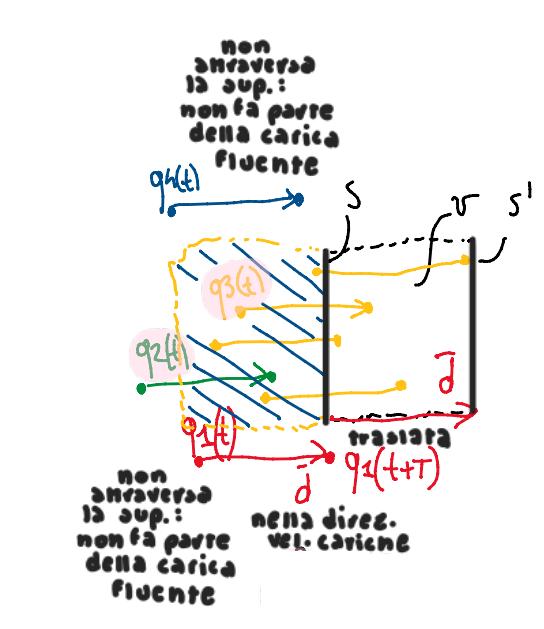
\includegraphics[scale=0.5]{immagini/image2.png}
\end{center}
\[
    q^f[T,S] = \int_v \rho_cdv = \rho_c \int_v dv = \rho_cv = \rho_cS(\overline{d}\cdot\hat{n}) = \rho_c \overline{v}\cdot\hat{n}ST
\]
\[
i[t,s] = \lim_{T \to 0} \frac{\rho_c \overline{v}\cdot\hat{n}S\not{T}}{\not{T}} = \rho_c\overline{v}\cdot\hat{n}S
\]
Si denota con $\overline{J} = \rho_c\overline{v}$ la densità di corrente e si misura in $[\frac{A}{m^2}]$. Descrive localmente il moto delle cariche.


Per ottenere un modello più generale si devono rimuovere le ipotesi semplificative che sono state fatte.\\
\begin{enumerate}
    \item Superfici curve: ogni superficie infinitesima è piana
    \item $\mathbf{v}$, $\rho_c$ costanti. Per il \textbf{principio di uniformità}: posso ritenere $\mathbf{v}$, $\rho_c$ uniformi e costanti a patto di considerare $S\to0$ e $T\to0$
\end{enumerate}

Applicando il principio di uniformità l'espressione di prima è ancora valida se consideriamo gli infinitesimi:
\[
di[t,ds] = \overline{J}(t,P)\cdot\hat{n}ds
\]
con $ds$ superficie infinitesima centrata in $P$. Se si volesse considerare una superficie $\Sigma$ non infinitesima?
\[
    i[t,\Sigma] = \int_\Sigma\overline{J}(t,P)\cdot\hat{n}(P)ds
\]
\begin{center}
    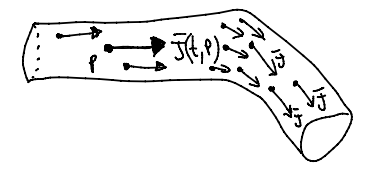
\includegraphics[scale = 0.6]{immagini/image3.png}
\end{center}

$\overline{J}$ è un campo vettoriale: torna un vettore in ogni punto $P$ del dominio.

\subsection{Come visualizzare i campi vettoriali}
\begin{center}
    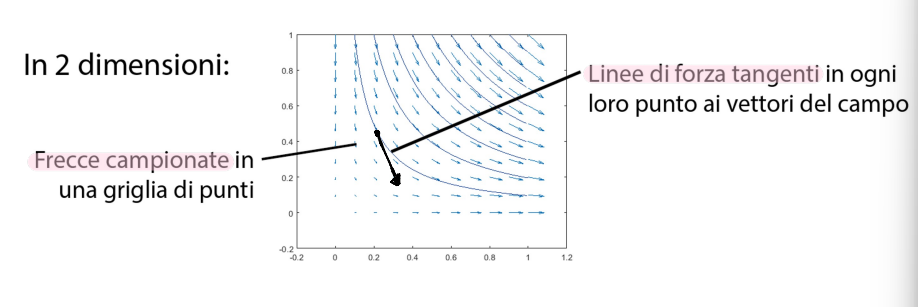
\includegraphics[scale = 0.6]{immagini/image4.png}
\end{center}
Due linee di forza ovviamente non possono sovrapporsi in quanto in un punto $Q$ è presente solo un vettore.
\subsubsection{Conduttore filiforme}
    \begin{center}
        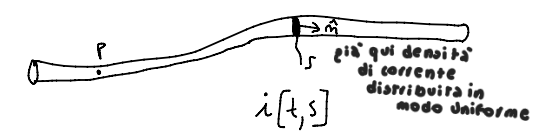
\includegraphics[width=0.5\linewidth]{immagini/image6.png}    
    \end{center}
    d è il diametro della sezione e l la lunghezza, si considera l>>d.\\
    In queste condizioni la sezione S è talmente piccola da ritenersi quasi infinitesima ed è possibile applicare il \textbf{principio di uniformità}
    \begin{center}
        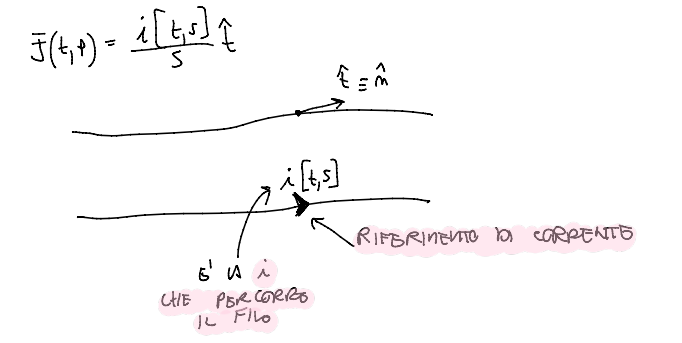
\includegraphics[width=0.5\linewidth]{immagini/image5.png}  
    \end{center}

\subsection{Legge di continuità della carica elettrica}
    Il principio di conservazione della carica: la carica non si crea e non si distrugge in quantità macroscopica.

    Il \textbf{bordo} del volume $v$ è una superficie $S=\partial v$. $\partial v$ sono superfici \textbf{chiuse}, cioè $\partial S = \partial\partial v = 0$.

    L'obiettivo è mettere in relazione la carica contenuta in $v$ con la carica fluente dal suo bordo. La variazione di carica contenuta corrisponde alla carica fluita all'esterno del volume.
    \[
        q^f[t,\partial v] = q^c[t,v] - q^c[t+T,v]
    \]
    Cariche fluite attraverso il volume = differenza di carica tra l'inizio (t) e la fine dell'intervallo (t+T)
    \[
        q^f[T,\partial v] = \int_T i[t,\partial v]dt = i[t, \partial v]\cdot T
    \]
    $i$ è costante per $T\to0$\\
    Ricavo la $i$
    \[
        i[t,\partial v] = \lim_{T\to0} \frac{q^c[t,v] - q^c[t+T, v]}{T} = \lim_{T\to0} -\frac{q^c[t+T,v]- q^c[t,v]}{T}=
    \]
    \[
        = -\frac{dq^c[t,v]}{dt} = \lambda[t,\partial v]
    \]

    Ricaviamo ora la formula differenziale, cioè con variabili puntuali
    \[
        i[t,\partial v] = \int_{\partial v}\overline{J}\cdot\hat{n}ds = -\frac{d}{dt}\{\int_v \rho_cdv\}
    \]
    $i$ è il flusso di $\overline{J}$ su una superficie  e $\int_v \rho_c dv$ corrisponde a $q^c[t,v]$.

    Per procedere dobbiamo trasformare l'integrale di superficie in uno di volume. Si usa il teorema della \textbf{divergenza}:
    \[
        \oint_{\partial v}\overline{u}\cdot\hat{n}ds = \int_v \nabla \overline{u}dv
    \]
    Quindi
    \[
        \int_v \nabla \overline{J}dv = -\frac{d}{dt}\int_v \rho_cdv = \int_v - \frac{\partial \rho_c(t,P)}{\partial t} dv
    \]
    \[
        \int_v (\nabla \overline{J} + \frac{\partial \rho_c}{\partial t})dv = 0
    \]
    Che  $\forall\tau \subseteq v$ vale la stessa relazione
    \[
        \int_\tau (\nabla \overline{J} + \frac{\partial \rho_c}{\partial t})dv = 0
    \]

    Dato che l'integrale vale 0 $\forall \tau$ si può dedurre che l'argomento è nullo:
    \[
     \nabla \overline{J} = -\frac{\partial \rho_c}{\partial t}
    \]

    Cos'è la divergenza dal punto di vista fisico.
    \[
    \nabla \overline{J}(t, P) = \lim_{v \to 0} \int_{\partial v}\frac{ \overline{J}(t, P) \cdot \hat{n}ds}{v} = \lim_{v \to 0} \frac{i[t,\partial v]}{v}
    \]

Se in un punto $\nabla \overline{J}(t, P) = 0$, nel punto $P$ non nasce una corrente.\\

Se in un punto $\nabla \overline{J}(t, a) > 0$. Nel punto a nasce una \textbf{corrente sorgente}\\

Se in un punto $\nabla\overline{J}(t, b) < 0$, i punti in cui ciò accade si chiamano \textbf{pozzi} (muore una corrente).

consideriamo ora il caso $\nabla\overline{J} = 0 \Rightarrow \overline{J}$ solenoidale (o conservativo.\\
Quando $\overline{J}$ è solenoidale?

a) $\overline{v}= 0$ , cariche ferme. $\Rightarrow \overline{J} = \rho_c\overline{v} = 0 \Rightarrow \nabla \overline{J} = 0$. \textbf{Elettrostatica}

b) $\overline{J}, \overline{v}$ per ipotesi costanti implica $\rho_c$ costante e ovviamente deriva $\frac{\partial \rho_c}{\partial t} = 0 \Rightarrow \nabla\overline{J} = 0$. \textbf{Conduzione stazionaria} (casi in cui è circa pari a zero, caso campo quasi-stazionario)

c) se $\frac{\partial \rho_c}{\partial t} = 0$ ma $\overline{v} \,\text{e}\ \overline{J}$ variano.
\subsubsection{Proprietà campi solenoidali}
1) Non ci sono né pozzi e né sorgenti. Le linee di forza del campo vettoriale $\overline{J}$ sono linee chiuse (si richiudono per forza su se stesse)

2) \begin{itemize}
    \item prendiamo una superficie S
    \item consideriamo tutte le linee di forza di $\overline{J}$ che intersecano S
    \begin{center}
        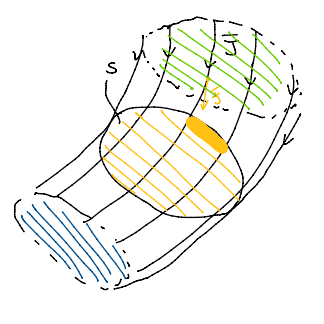
\includegraphics[scale=0.7]{immagini/image7.png}
    \end{center}

    Risulta un fascio di linee di forza. Il volume occupato dal fascio si chiama \textbf{tubo di flusso}
    \item consideriamo solo un pezzo del tubo di flusso. è caratterizzato da due superfici "tappo" ($S_A$ e $S_B$)
    \item $\nabla \overline{J} = 0 \Rightarrow \int_{\partial \tau}\overline{J}\cdot\hat{n}ds = 0$ con $\tau$ normale che esce dal volume\\
    \[\int_{S_A}\overline{J_A}\cdot\hat{n_A}ds + \int_{S_B}\overline{J_B}\cdot\hat{n_B}ds + \cancel{\int_{S_l}\overline{J_l}\cdot\hat{n_l}ds} = 0\]
    L'ultimo termine vale zero in quanto ortogonali i termini all'interno dell'integrale.\\
    Definendo $\hat{n_{B'}} = -\hat{n_B}$ e sostituendo
    \[
        \int_{S_A} \overline{J_A} \cdot \hat{n}_A \, ds - \int_{S_B} \overline{J_B} \cdot \hat{n}_{B'} \, ds = 0 \Rightarrow i_A[t, S_A] = i_B[t,S_B]
    \]
    \end{itemize}

\section{Campo elettrostatico – Campo elettrico coulombiano}
Partendo dalle ipotesi:
\begin{itemize}
    \item \textbf{Elettrostatica} (cariche ferme, non in movimento)
    \item \textbf{Mezzo nella regione di studio}:
   Omogeneo, lineare, isotropo (stesse proprietà fisiche in ogni direzione).
\end{itemize}

\subsection{Legge sperimentale di Coulomb}
    \[
        \overline{F}_{q0} = \frac{1}{4\pi\epsilon}\frac{q\cdot q_0}{r^2}\hat{u}'
    \]
    Indica la forza agente su $q_0$ dovuta alla presenza di q.\\

    \textbf{Campo elettrostatico $\overline{E}_c(P)$}: è una \textbf{forza elettrica specifica} ovvero di natura elettrica e per unità di carica
    \[
        \overline{E}_c(P) := \lim_{q_0 \to 0} \frac{\overline{F}_{q_0}}{q_0} = \frac{1}{4\pi\epsilon}\frac{q}{r^2}\hat{u}
    \]
    Questo modello ha significato se ci si trova sufficientemente lontani dalla carica in quanto essendo un modello dipendente dalla distanza come $\frac{1}{r^2}$, se essa tende a 0, il campo tende a infinito.
    \[
        \overline{F}_{q0} = q_0 \vec{E_c}(t), \quad [E_c] = [V]
    \]

\subsection{Proprietà del campo elettrostatico}

1) Non è solenoidale.

2) È un campo conservativo:

\[
\oint_{l_c} \vec{E_c} \cdot \hat{t}\,dl = 0 \quad \forall l_c
\]

\paragraph{Teorema di Stokes (o del rotore)}:

\[
\oint_{\gamma} \vec{E} \cdot \vec{dl} = \int_S (\nabla \times \vec{E}) \cdot \vec{dS}
\]
\begin{center}
    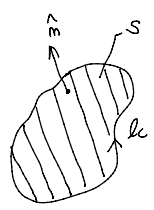
\includegraphics{immagini/image8.png}
\end{center}
a) $\partial S = l_c$\\
b) S non è unica\\
c) l'orientamento di S non si può scegliere a caso ma si ottiene a partire da $l_c$ con la regola della mano destra.\\

Applicando il teorema di Stokes:

\[
\oint_{l_c} \vec{E_c} \cdot \hat{t}\,dl = \int_S (\nabla \times \vec{E_c}) \cdot \hat{n}\,ds \quad \forall l_c
\]

Essendo l'integrale nullo per ogni $l_c$, il rotore del campo è nullo:

\[
\nabla \times \vec{E_c} = 0
\]

Il rotore è sempre nullo $\Rightarrow$ \textbf{campo irrotazionale}.

3) L'integrale di linea di $\vec{E_c}$ tra due punti $A$ e $B$ non dipende dal percorso:
\begin{center}
    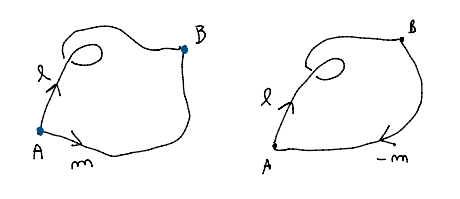
\includegraphics{immagini/image9.png}
\end{center}
\[
    \oint_{lc} \vec{E_c} \cdot \hat{t}dl = \int_{l} \vec{E_c} \cdot \hat{t}dl - \int_{m} \vec{E_c} \cdot \hat{t}dl
\]
\[
    \int_{l} \vec{E_c} \cdot \hat{t}dl = \int_{m} \vec{E_c} \cdot \hat{t}dl
\]
4) Proprietà del campo irrotazionale:

\[
\nabla \times (\nabla V) = 0, \quad \forall V \text{ scalare}
\]

Possiamo introdurre un \textbf{potenziale}: una variabile fisica ausiliare che serve a rappresentare una grandezza fisica che verifica implicitamente una legge.

\[
\nabla \times \vec{E_c} = 0
\]
ricordando che 
\[
    \vec{E_c} = -\nabla V
\]
Il campo scalare V è detto \textbf{potenziale elettrostatico}.\\
Trovando l'integrale di linea di $\vec{E_c}$ su l:

\[
\int_{A,l}^B \vec{E_c} \cdot \hat{t} dl = \int_{A,l}^B -\nabla V \cdot \hat{t} dl = V(A) - V(B)
\]
Questa soluzione deriva dal teorema del gradiente.

\subsection{Trovare V(P) da una singola carica puntiforme}

\begin{center}
    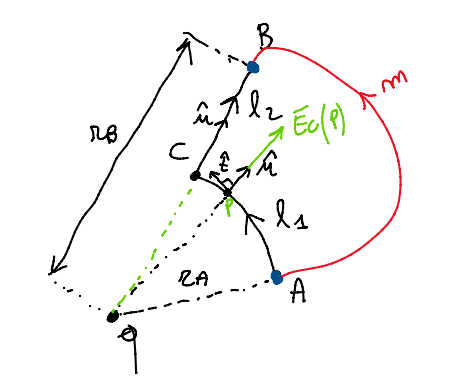
\includegraphics[scale = 0.7]{immagini/image10.png}
\end{center}

\[
\int_{A}^{B} \vec{E}_c \cdot \hat{t}  \, dl = \int_{A,l1}^{C} \vec{E}_c \cdot \hat{t}  \, dl + \int_{C,l2}^{B}\vec{E}_c \cdot \hat{t}  \, dl
\]

\[
\int_{A,l1}^{C} \vec{E}_c \cdot \hat{t}  \, dl = \int_{A,l1}^{C} \frac{q}{4 \pi \epsilon} \cdot \frac{1}{r^2_A} \cdot \hat{u} \cdot\hat{t}  \, dl = 0
\]

\[
\int_{C,l2}^{B} \vec{E}_c \cdot \hat{t}  \, dl = \int_{C,l2}^{B} |\vec{E}_c| \cdot \frac{\vec{E}_c}{|\vec{E}_c|} \cdot \hat{t}  \, dl = \int_{C}^{B} |\vec{E}_c|  \, dl = \int_{r_A}^{r_B} \frac{q}{4 \pi \epsilon} \cdot \frac{1}{r^2} dr = \frac{q}{4\pi\epsilon}(\frac{1}{r_A}-\frac{1}{r_B}) = V(A)-V(B)
\]

Imponendo le condizioni all'infinito
\[
\lim_{r\to\inf}V(P)=0 = \lim_{r\to\inf}(\frac{q}{4\pi\epsilon}\frac{1}{r} + c)  = 0+c = 0
\]

La D.D.P. non dipende dalla costante.\\
Nel momento in cui sono presenti più cariche si può sfruttare il principio di \textbf{sovrapposizione degli effetti}.\\

Non in elettrostatica si definisce l'analogo di $\vec{E}_c$ che è
\[
    \vec{E}(t,P) = \lim_{q_0\to 0}\frac{\vec{F}_{q0}(t,P)}{q_0}
\]
\[
    \vec{E}(t,P) = \vec{E}_c(t,P) + \vec{E}_i(t,P)
\]
Con $\vec{E}_i(t,P)$ campo elettrico indotto.\\

\[\nabla \vec{E} = \nabla \vec{E}_i \not= 0\]

Questo porta a dire che $\vec{E}$ non è irrotazionale e consegue che non è possibile definire V e l'integrale di linea dipende dal percorso.


L'integrale di linea di $\vec{E}$ è detta \textbf{tensione} u. È una variabile globale:
\[
u[t,l] = \int_{A,l}^B\vec{E}(t,P)\cdot\hat{t} \, dl
\]
\subsection{Campo elettrostatico e potenziale generato da distribuzioni di carica}

Ipotesi: la distribuzione della carica è nota, ad esempio è nota la densità volumica di carica $\rho_c(P)$.

Allora esistono formule analitiche per trovare $\vec{E_c}$ e $V$ in ogni punto dello spazio:

\[
\vec{E_c}(\vec{r}) = \int_{v} \frac{\rho_v (Q)}{4\pi \varepsilon r^2} \hat{u} \, dv
\]

\[
V(P) =\int_{v} \frac{\rho_v (Q)}{4\pi \varepsilon r}\, dv
\]

\[
V = \frac{1}{4\pi \varepsilon_0} \cdot \frac{q}{r}
\]

\section{Il fenomeno fisico della conduzione elettrica}
Ipotesi:\\
Condizione stazionaria ($\vec{J} costante, \nabla\vec{J} = 0, \vec{E} = \vec{E}_c$)
\subsection{Esperimento di Ohm}
Cambiare la batteria registrando i valori di i e u. Si verifica sperimentalmente che $\frac{u}{i}$ = costante.\\
La II° legge di Ohm: $R = \rho \frac{l}{s}$ con $\rho$  resistività del materiale (da non confondere con la densità volumetrica di carica).\\

La R dipende ovviamente dalla temperatura, si introduce quindi un \textbf{coefficiente di temperatura $\alpha$}
\[
    \rho(t_0+\theta) = p(t_0)(1+\alpha\theta)
\]
con $t_0 + \theta$ temperatura alla quale voglio valutare la resistività

\subsection{Effetto Joule}

Si misura con un calorimetro il calore $Q$ prodotto dal passaggio di corrente nel provino, esce che:
\[
Q = R i^2T
\]
Il calore dissipato $Q$ per effetto Joule è pari al lavoro elettrico assorbito dal provino
\[
\mathcal{L}_e = Q
\]
\begin{center}
    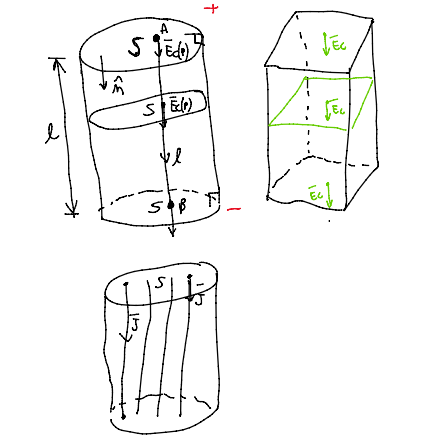
\includegraphics[scale = 0.5]{immagini/image11.png}
\end{center}
Si prende il provino e si seziona in superfici tutti uguali e piane, i campi quindi risultano uniformi all'interno del provino.
\[
u = \int_{A,l}^{B} \vec{E}_c \cdot \hat{t}  \, dl = \int_{A,l}^{B} |\vec{E}_c| \cdot \frac{\vec{E}_c}{|\vec{E}_c|} \cdot \hat{t}  \, dl = |\mathbf{E}_c|  \int_{A,l}^{B}\hat{u}\cdot\hat{t}dl = |\vec{E}_c|\cdot l
\]
\[
i = \int_S \vec{J}\cdot\hat{n} \, ds = |\vec{J}|\cdot S
\]
Sostituendo si arriva a dire che
\[
    \vec{E}_c = \rho\vec{J}
\]

\subsection*{Applicazioni dell'effetto Joule}

Si sfrutta per il riscaldamento: stufe a filo (non pompa di calore), piastra della cucina elettrica (non a induzione).

Nella maggior parte dei casi però l'effetto Joule è indesiderato perché provoca il riscaldamento dell'elettronica e dei fili percorsi da corrente. Questo produce due problemi:

1) Potenza dissipata inutile
2) Se il calore non viene dissipato, la temperatura aumenta. Questo è un problema molto grave che non permette l'ulteriore riduzione delle dimensioni dell'elettronica.

\subsection{Superfici di discontinuità della resistività}
\begin{center}
    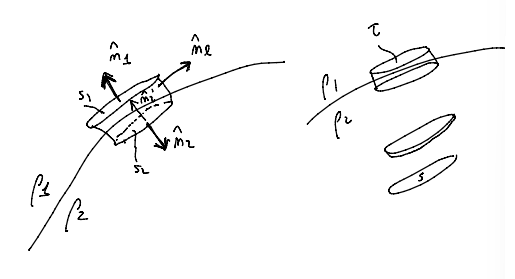
\includegraphics[scale = 0.6]{immagini/image12.png}
\end{center}
Si considera un volume $\tau$ a cavallo dell'interfaccia, S1,S2 sono le superfici "tappo" e le prendiamo uguali e infinitesime. La superficie laterale di $\tau$ è un infinitesimo di ordine superiore rispetto a S quindi risulta trascurabile.

\[
\int_{S1} \vec{J_1}\cdot\hat{n}_1 \, ds + \int_{S2} \vec{J_2}\cdot\hat{n}_1 \, ds + \cancel{\int_{Sl} \vec{J_l}\cdot\hat{n}_l \, ds} = -\frac{d}{dt}\int_S\sigma_cds
\]     
Per il principio di uniformità:
\[
    \vec{J}_1\cdot\hat{n}_1\cancel S + \vec{J}_2\cdot\hat{n}_2\cancel S = -\frac{\partial \sigma_c}{\partial t}\cancel S
\]
cambiando il riferimento per il secondo termine (cambio il segno) si ottiene alla fine che se
\[
-\frac{\partial \sigma_c}{\partial t} = 0 \Rightarrow \vec{J}_1\cdot\hat{n}_1 = \vec{J}_2\cdot\hat{n}_2'
\]

Si può fare il caso analogo prendendo una linea chiusa e ripetere il procedimento con il campo Elettrostatico. Si arriva a dedurre che: $\vec{E}_{C1} \cdot \hat{t}_1 = \vec{E}_{C2} \cdot \hat{t}_2$
\section{Bilancio locale di potenza}
\[
 P_d = R i^2 = (\rho\frac{l}{s})|\vec J|^2 s^2 = \rho |\vec J|^2v
\]
$v$ risulta il volume del cilindro dato dalla superficie per il lato.\\
Consideriamo un volume infinitesimo centrato in un punto P. Posso definire la densità di potenza dissipata:
\[
pd(t,P) = \lim_{v\to0}\frac{P_{d,v}}{v} = \rho J^2(t,P) = \vec E_c\cdot\vec J = pe(t,P)
\]
Si usa la minuscola per la densità, per indica la densità di potenza elettrica.
\subsection{forze elettriche specifiche F.E.S generatrici}
Alcune delle FES più importanti non di natura elettrica sono la pila: di natura chimica, una turbina: di natura meccanica. Vogliamo avere la risultante delle FES: FES totale $\vec E t$ che è la somma di una parte di natura elettrica e una non elettrica. 

\section{Bilancio di potenza esteso a tutto il dominio}
Ci poniamo nell'ipotesi di conduzione stazionaria. Prendiamo $\tau_J$ volume tale in cui $\vec J \not = 0$, scriviamo il bilancio di potenza su tale volume e integriamo il bilancio di potenza locale sullo stesso.
\[\rho J^2(P) = \vec E_t(P) \cdot \vec J (P)\]
\[
\int_{\tau_J} \rho J^2dv = \int_{\tau_J} \vec E_t \cdot \vec J dv = \int_{\tau_J} \vec E_c \cdot \vec J dv + \int_{\tau_J} \vec E_g \cdot \vec Jdv
\]
Usando l'identità vettoriale:
\[
    \nabla (V\vec J) = V \nabla  (\vec J) +gradV \cdot\vec J = -\vec E_c \vec J
\]

Studiando la componente elettrica:
\[
\int_{\tau_J} \vec E_c \cdot \vec J dv = - \int_{\tau_J}\nabla(V\vec J) dv = 0
\]
Dato che $\vec E_c$ è conservativo, non compie lavoro su percorsi chiusi come sono le linee di $\vec J$. Generalmente non compie lavoro e sono necessarie FES generatrici.

\[
    \int_{\tau_J}\rho J^2dv = \int_{\tau_J}\bar Eg\cdot\bar Jdv 
\]
Risulta che la potenza dissipata (primo termine) per effetto Joule sia uguale alla potenza generata da altre forme di energia (chimica, ecc.)

Calcoliamo ora:
\[
    \int_\tau \bar Ec \cdot \bar J dv = -\int_{\partial \tau}V \bar J \cdot \hat{n}ds
\]
\[
= \cancel{\int_{sl}V \bar J \cdot \hat{n}ds} - {\int_{SA}V \bar J \cdot \hat{n}ds} - {\int_{SB}V \bar J \cdot \hat{n}ds} \not = 0
\]
\begin{center}
    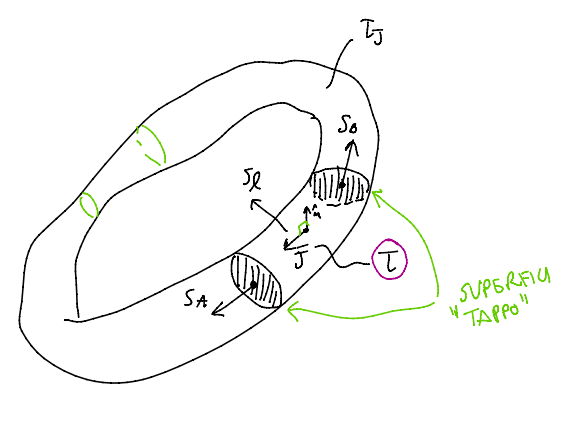
\includegraphics[scale = 0.5]{immagini/image13.png}
\end{center}
Il contributo di $\bar Ec$ su $\tau$ non è nullo. È determinante per trasferire potenza dentro $\tau_J$
\[
P_{d,\tau} = P_{g,\tau} + \int_\tau\bar Ec \cdot \bar J dv \Rightarrow P_{g,\tau} - P_{d,\tau} = - \int_\tau\bar Ec \cdot \bar J dv
\]
Risulta che la potenza dissipata è la potenza generata + la componente dell'integrale

\section{Modelli circuitali per la conduzione stazionaria}
    Modello circuitale: è una descrizione semplificata del fenomeno fisico. Per esempio nel modello di Ohm si usa solo la R in quanto interessa solo la relazione Tensione/Corrente.

    In forma generica si può calcolare la R di un conduttore. Per ipotesi si è in conduzione stazionaria ($\nabla\bar J = 0$). Consideriamo $\bar J$ tangente al bordo conduttore per canalizzazione. Questo va a denotare una porzione del tubo di flusso di $\bar J$. La corrente nel conduttore è la stessa per ogni superficie che taglia il tubo di glusso e si può quinid associare una corrente $i$ al conduttore

    \begin{center}
        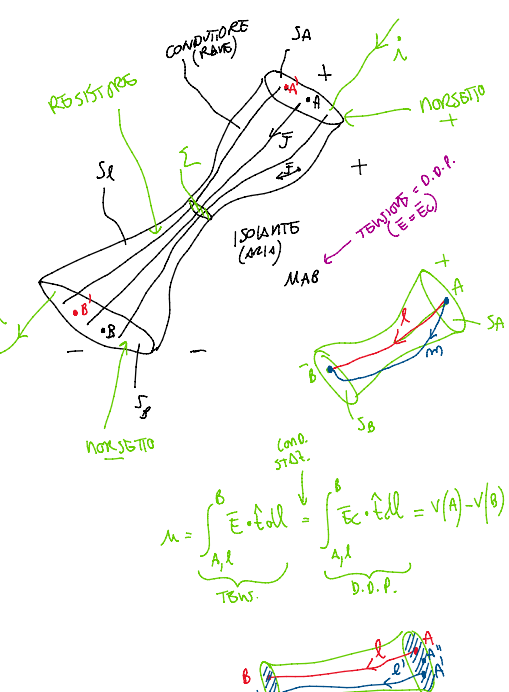
\includegraphics[scale = 0.5]{immagini/image14.png}
    \end{center}

    \subsection{Resistore}
        Ipotesi: $\bar E_t = \bar E_c$\\
        Vogliamo parlare anche di tensione ai capi del conduttore/componente. La tensione è $u = D.D.P$ in quanto regime stazionario.
        \[
            u_{AB} = \int_{A,l}^B \bar E_c \cdot\hat{t} dl
        \]
        Avere questo si deve assumere per ipotesi che $S_a$, $S_B$ siano equipotenziali. Facendo ciò si può parlare di $u$ sul componente. Si introduce la resistenza come: $R = \frac{u_{AB}}{i}$

        Con questo componente si utilizza la convenzione dell'utilizzatore: Pendo la corrente in modo che entri dal morsetto positivo.
        
        INSERIRE SCHEMI RESISTENZE

        \subsubsection{Calcolo della resistenza}
        \paragraph{Resistore filiforme}
            l è la lunghezza e si considera l>>d
            \[
            R = \frac{u}{i}
            \]
            
            \noindent
            Posso assumere $\vec{J}$ uniforme su $S$.
            
            \[
            i = \int_S \vec{J} \cdot \hat{n}\, dS = J \cdot S
            \]
            
            \noindent
            Assumendo di avere simmetria piana:
            
            \[
            u = \int_{A,l}^B \vec{E_c} \cdot \hat{t}\, dl \simeq E_C \, l = \rho J l
            \]
            \[
            \text{(Ipotesi: } |\vec{E}| \text{ uniforme)}
            \]
            
            \[
            E_c = \rho J
            \]
            
            \[
            R = \frac{u}{i} = \frac{\rho J l}{J S} = \rho \frac{l}{S} \simeq R
            \]
        \paragraph{Resistore cilindrico}
        \textbf{Simmetria cilindrica}
        \begin{center}
            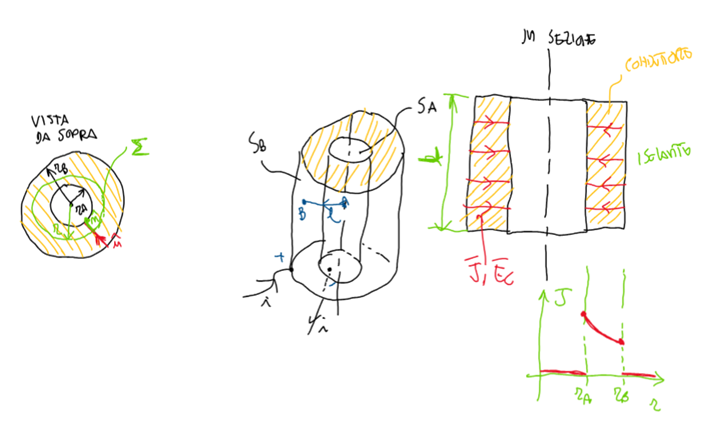
\includegraphics[scale = 0.5]{immagini/image15.png}
        \end{center}
        
        \[
        i = \int_{\Sigma} \vec{J} \cdot \hat{n}\, dS 
           = |\vec{J}| \int_{\Sigma} \hat{u} \cdot \hat{n}\, dS
           = J \Sigma = J (2 \pi r\, l)
        \]
        
        \[
        J = \frac{{i}}{2 \pi r\, l}
        \]
        
        \[
        E_c = \rho J = \frac{\rho{i}}{2 \pi r\, l}
        \]
        
        \[
        u = \int_{A,l}^{B} \vec{E_c} \cdot \hat{t}\, dl 
             = \int_{r_A}^{r_B} \frac{\rho {i}}{2 \pi r\, l}\, dr
             = \frac{\rho i}{2 \pi l} \int_{r_A}^{r_B} \frac{1}{r}\, dr
             = \frac{\rho i}{2 \pi l} \ln{\left( \frac{r_B}{r_A} \right)} = R
        \]


\paragraph{Resistore sferico}

\[
i = \int_{\Sigma} \vec{J} \cdot \hat{n}\, dS 
  = J \int_{\Sigma} \hat{u} \cdot \hat{n}\, dS 
  = J \, \Sigma 
  = J \, (4 \pi r^2)
\]

\[
J(r) = \frac{i}{4 \pi r^2}
\]

\[
E_c = \rho J = \frac{\rho \, i}{4 \pi r^2}
\]

\[
u = \int_{A,l}^{B} \vec{E_c} \cdot \hat{t}\, dl 
    = \int_{A,l}^{B} E_c \, dl 
    = \int_{r_A}^{r_B} \frac{\rho \, i}{4 \pi r^2} \, dr
\]

\[
u = \frac{\rho \, i}{4 \pi} 
       \int_{r_A}^{r_B} \frac{1}{r^2} \, dr
     = \frac{\rho \, i}{4 \pi} 
       \left( \frac{1}{r_A} - \frac{1}{r_B} \right)
\]

\[
R = \frac{u}{i} 
  = \frac{\rho}{4 \pi} 
    \left( \frac{1}{r_A} - \frac{1}{r_B} \right)
\]
1) Metà sfera\\
2) $r_B\to \infty$\\
Implica che 
\[
    R_T = \frac{\rho}{4\pi}\cdot\frac{1}{r_A}\cdot2 = \frac{\rho}{2\pi}\cdot\frac{1}{r_A}
\]
        

            
\section{Come trovare $R$ nel caso generale}

\textbf{Come risolvere problemi di conduzione stazionaria}

\[
\begin{cases}
\mathrm{div}\,\vec{J} = 0 \\
\vec{E_c} \text{ conservativo } \Rightarrow \vec{E_c} = -\nabla V \\
\vec{E_c} = \rho \vec{J}, \quad \vec{J} = \gamma \vec{E_c}
\end{cases}
\]

\[
\mathrm{div}\,\vec{J} = \mathrm{div}(\gamma \vec{E_c}) 
   = -\,\mathrm{div}(\gamma \nabla V) = 0
\]

\[
\text{(Equazione di Laplace)}
\]

\[
\text{Se ho lo stesso materiale (omogeneo)} 
   \Rightarrow \gamma = \text{costante} 
   \Rightarrow \mathrm{div}(\nabla V) = \nabla^2 V = 0
\]

\[
\boxed{\nabla^2 V = 0}
\]
\begin{center}
    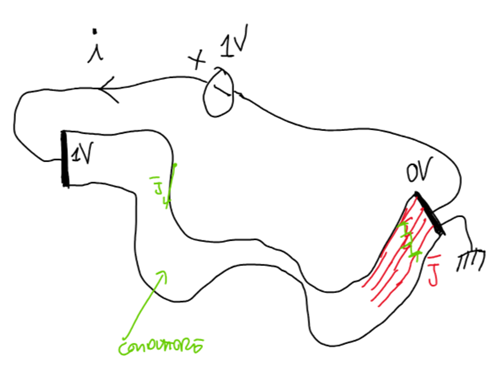
\includegraphics[scale = 0.5]{immagini/image16.png}
\end{center}
\subsection*{Bisogna specificare le condizioni al contorno}

\begin{enumerate}
    \item \textbf{Condizione di Dirichlet:} assegno il valore di $V$ su tutto il bordo.  
    \hfill (soluzione unica)
    
    \item \textbf{Condizione di Neumann:} assegno il valore di $\dfrac{\partial V}{\partial n}$ su tutto il bordo.  
    \hfill (infinite soluzioni in $V$ $\vec{E_c} = -\nabla V$)

    \item \textbf{Condizione “mista”} la soluzione è unica.
\end{enumerate}

\subsection*{Dal punto di vista fisico}
\begin{enumerate}[label=\alph*)]
  \item I morsetti sono \textbf{equipotenziali}.
  \item D.D.P. tra i morsetti è fissata (1V) $\Rightarrow \text{Applico condizioni di Dirichlet sui morsetti.}$
  \item  Sulla parte restadnte di bordo: $\vec{J} \cdot \hat{n} = J_n = 0$
\end{enumerate}

Le soluzioni del problema di Laplace sono dette \textbf{funzioni armoniche}.  
Il valore o i minimi di queste funzioni stanno su $\partial V$.

\[
\begin{cases}
\mathrm{div}\,\vec{E_c} = 0 \\[6pt]
\mathrm{rot}\,\vec{E_c} = 0
\end{cases}
\]

\[
\oint_{l_c} \vec{E_c} \cdot \hat{t}\, dl = 0 
\quad \Longleftrightarrow \quad 
\mathrm{rot}\,\vec{E_c} = 0
\]

\begin{center}
    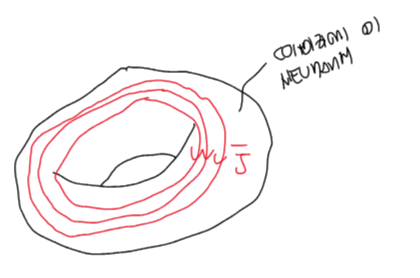
\includegraphics[scale = 0.7]{immagini/image17.png}
\end{center}

\section{Componente: Generatore elettrico}

È una porzione del tubo di flusso di $\vec{J}$, dove: $\vec{E_t} = \vec{E_c} + \vec{E_g}$

\begin{enumerate}
  \item $\vec{E_g}$ provoca una separazione di carica sui morsetti.
  \item Con la separazione di carica si genera un campo $\vec{E_c}$.
\end{enumerate}

\paragraph{Caso 1:} 
\textit{“A vuoto”} non connettiamo nulla al generatore che faccia scorrere una corrente.

\medskip
Quando si realizza l’equilibrio, le cariche restano ferme $\Rightarrow$ \textbf{elettrostatica.}

\[
\vec{E_t} = \rho \vec{J} = \rho \cdot 0 = 0 = \vec{E_c} + \vec{E_g}
\]

\[
\boxed{\vec{E_c} = -\vec{E_g}}
\]

se connettiamo il voltmetro ai capi del generatore:
\[
u_V = \int_{B,l_{EST}}^A \vec{E_t} \cdot \hat{t}\, dl 
    = \int_{B,l_{INT}}^A \vec{E_c} \cdot \hat{t}\, dl
    = \int_{B,l_{INT}}^A (-\vec{E_g}) \cdot \hat{t}\, dl 
    = \int_{A,l_{INT}}^B \vec{E_g} \cdot \hat{t}\, dl = e_{BA} = u_{BA}
\]
\noindent
\textit{(lettura del voltmetro)}  
\[
\text{Forza elettromotrice (FEM) del generatore:} \quad
e_{BA} = \int_A^B \vec{E_g} \cdot \hat{t}\, dl
\]
\[
\mu_{BA} = \int_B^A \vec{E_c} \cdot \hat{t}\, dl, 
\quad \text{e } \quad \mu_{BA} = e_{BA}
\]
\begin{center}
    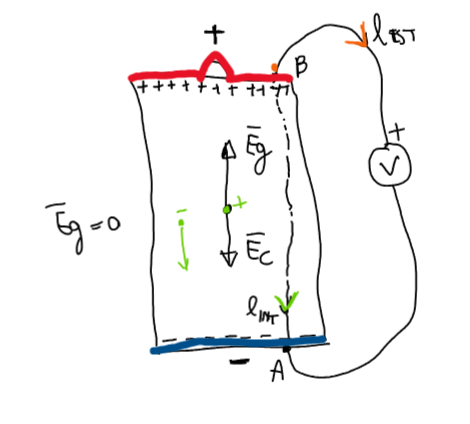
\includegraphics[scale = 0.7]{immagini/image18.png}
\end{center}

\subsection{Caso 2:}
“A carico” il generatore eroga una corrente $i$.

\[
\vec{E_t} = \rho \vec{J} = \vec{E_c} + \vec{E_g} \neq 0
\]

\[
R = \frac{1}{i} \int_A^B \vec{E_t} \cdot \hat{t}\, dl 
  = \frac{1}{i} \left( \int_A^B \vec{E_c} \cdot \hat{t}\, dl 
  + \int_A^B \vec{E_g} \cdot \hat{t}\, dl \right)
\]

\[
R = \frac{u_{AB} + e_{BA}}{i}
  = \frac{u_{BA} + e_{BA}}{i}
\]
\[
u_{BA} = e_{BA} - Ri
\]

\subsection{Bilancio di potenza nei generatori}
    \[
        Pe = u_{BA} \cdot i = (e_{BA} - Ri)\cdot i = e_{BA}i - Ri^2
    \]
    La potenza erogata è pari alla potenza generata meno la potenza dissipata per effetto Joule sulla R, nel caso di un GIT la dissipazione di potenza sulla resistenza è nulla (non c'è R).
\section{N-Poli}
    Gli N-Poli sono componenti con N morsetti, si può vedere come un tratto di tubo di flusso di $\vec{J}$ ramificato.
    \subsection{Proprietà}
        Siamo in \textbf{conduzione stazionaria} $\;\Rightarrow\; \mathrm{div}\,\vec{J}=0$ 

\[
\oint_{\partial V}\vec{J}\cdot\hat{n}\,dS=0
= \int_{S_L}\vec{J}\cdot\hat{n}\,dS
  + \sum_{j=1}^{N}\int_{S_j}\vec{J}\cdot\hat{n}_j\,dS
\]
\emph{$\vec{J}$ tangenziale su $S_L$. \;($S_j$ = superfici dei \textit{morsetti})}

\subsection*{3-polo (caso generale $N$)}
\[
\sum_{j=1}^{N} i_j = 0
\]
\emph{($i_j$ = corrente uscente dal morsetto $j$-esimo).}

\subsection*{Applicazione al bipolo: $N=2$}
\[
i_1 + i_2 = 0
\qquad\Longrightarrow\qquad
i_1 = -\,i_2
\]

\subsection*{Porta elettrica}
\textbf{Definizione:} una coppia di \textit{morsetti} in cui la corrente che entra da un morsetto esce dall’altro.

\subsection*{$M$-bipolo}
È un $N$-polo, con N = 2M, in cui i morsetti sono raggruppati in $M$ \textit{porte}.

\paragraph{Esempio}
$N=4,\; M=2 \;\Rightarrow\;$ \textit{4-polo}, \textit{2-porte}.

\subsection{Potenza elettrica scambiata da $N$-polo e $M$-bipolo}

Troviamo la potenza \textbf{uscente} da un $N$-polo:

\[
P_{\text{usc}} = - \int_{\tau} \vec{E_c} \cdot \vec{J}\, dv 
               = \oint_{\partial \tau} V \, \vec{J} \cdot \hat{n}\, dS
\]

\[
= \cancel{\int_{S_L} V\,\vec{J}\cdot\hat{n}_l\, dS}
  + \sum_{j=1}^{N} \int_{S_j} V\,\vec{J}\cdot\hat{n}_j\, dS
\]

Poiché $\vec{J}$ è tangente su $S_L$: $\Rightarrow \int_{S_L} V\,\vec{J}\cdot\hat{n}\, dS = 0$

Se $S_j$ è la superficie equipotenziale del morsetto $j$-esimo, $V = V_j$ costante su $S_j$:

\[
P_{\text{usc}} = \sum_{j=1}^{N} 
V_j \int_{S_j} \vec{J}\cdot\hat{n}_j\, dS
\]

Definendo:
\[
i_j = \int_{S_j} \vec{J}\cdot\hat{n}_j\, dS
\quad \text{(corrente del morsetto $j$-esimo)}
\]

\[
\boxed{
P_{\text{usc}} = \sum_{j=1}^{N} V_j\, i_j
}
\]



\end{document}